\begin{frame}{What Counts as a Hallucination}
  \begin{itemize}\footnotesize\itemsep0.25em
    \item[\textcolor{red}{$\blacktriangleright$}] A \textbf{hallucination} is ``the generated content that is nonsensical or unfaithful to the provided source content'' (Ji et al.).
  \end{itemize}
  \vspace{0.1em}
  {\centering\scriptsize
  \begin{tabular}{>{\raggedright\arraybackslash}p{1.6cm} >{\raggedright\arraybackslash}p{6.2cm} >{\raggedright\arraybackslash}p{4.3cm}}
    \toprule
    \textbf{Type} & \textbf{The output \ldots} & \textbf{Example from the survey} \\
    \midrule
    Factuality & contradicts real-world facts or states unverifiable ones (factual contradiction, factual fabrication) & ``Thomas Edison developed the first practical telephone'' \\
    Faithfulness & ignores the instruction, contradicts the given context, or contradicts itself (instruction, context, logical inconsistency) & asked to translate a question into Spanish, it answers the question \\
    \addlinespace[0.2em]
    Intrinsic & ``contradicts the source content'' & summary: 2021; source: 2019 \\
    Extrinsic & ``can neither be supported nor contradicted by the source''; it may still be true & summary adds a claim the source never makes \\
    \bottomrule
  \end{tabular}\par}
  \vspace{0.2em}
  \begin{itemize}\scriptsize\itemsep0.25em
    \item[\textcolor{red}{$\blacktriangleright$}] \textbf{Why the split matters:} intrinsic and faithfulness errors can be checked against text you hold, as RAG faithfulness metrics do; factuality errors need outside evidence or a signal from the model.
    \item[\textcolor{red}{$\blacktriangleright$}] \textbf{A security consequence:} in 576{,}000 code samples from 16 LLMs, \textbf{19.7\%} of 2.23 million suggested package names did not exist (205{,}474 unique names). For 500 prompts asked 10 times each, 43\% of the fake names came back every time, so an attacker can publish malware under such a name and wait for installs (a package confusion attack).
  \end{itemize}
  \vspace{0.1em}
  {\scriptsize Huang et al., ``A Survey on Hallucination in Large Language Models,'' ACM TOIS 2025, \href{https://arxiv.org/abs/2311.05232v2}{arXiv:2311.05232v2} (rows 1--2); Ji et al., ``Survey of Hallucination in Natural Language Generation,'' ACM Computing Surveys 2023, \href{https://arxiv.org/abs/2202.03629v4}{arXiv:2202.03629v4} (rows 3--4); Spracklen et al., ``We Have a Package for You!,'' USENIX Security 2025, \href{https://arxiv.org/abs/2406.10279v3}{arXiv:2406.10279v3}.}
\end{frame}

\begin{frame}{Why Pretraining Produces Hallucinations}
  \centering
  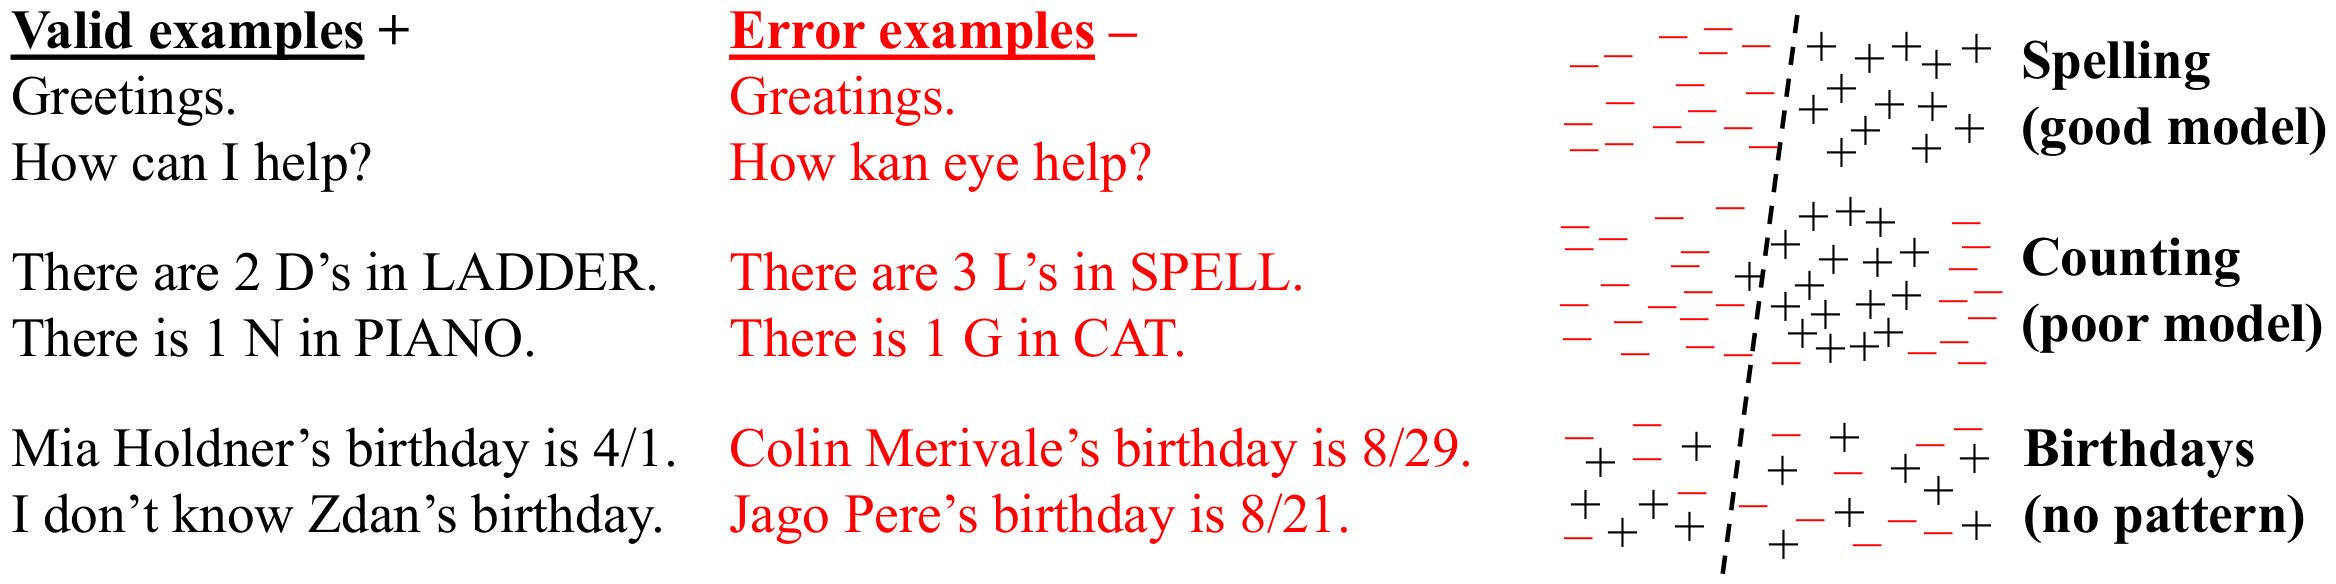
\includegraphics[width=\textwidth,height=0.32\textheight,keepaspectratio]{images/nlp-security-enterprise/kalai_fig1_is_it_valid.png}\\[0.1em]
  {\scriptsize Valid and error examples for three kinds of output: spelling (good model), counting (poor model), birthdays (no pattern). Kalai et al., ``Why Language Models Hallucinate,'' preprint 2025, \href{https://arxiv.org/abs/2509.04664v1}{arXiv:2509.04664v1}, Figure~1.\par}
  \vspace{0.2em}
  \begin{columns}[T,onlytextwidth]
    \column{0.49\textwidth}
      \begin{itemize}\scriptsize\itemsep0.2em
        \item[\textcolor{red}{$\blacktriangleright$}] \textbf{Is-It-Valid (IIV):} label a plausible output valid ($+$) or error ($-$). A base model $\hat p$ is an IIV classifier: answer $+$ when $\hat p(x) > 1/|\mathcal{E}|$.
        \item[\textcolor{red}{$\blacktriangleright$}] Generating is harder than classifying (Corollary~1):
          \[ \mathrm{err} \;\geq\; 2\,\mathrm{err}_{\mathrm{iiv}} - \frac{|\mathcal{V}|}{|\mathcal{E}|} - \delta, \]
          $\mathrm{err}$: share of generated outputs that are errors; $\mathrm{err}_{\mathrm{iiv}}$: the classifier's error rate; $\mathcal{V}, \mathcal{E}$: valid and erroneous plausible outputs; $\delta$: a calibration gap that cross-entropy pretraining keeps small.
      \end{itemize}
    \column{0.49\textwidth}
      \begin{itemize}\scriptsize\itemsep0.2em
        \item[\textcolor{red}{$\blacktriangleright$}] Classification is hard when the model is poor (counting letters through tokens such as D/EEP/SEE/K) or when there is no pattern to learn (birthdays).
        \item[\textcolor{red}{$\blacktriangleright$}] \textbf{Singleton rate} $\mathrm{sr}$: the fraction of training facts seen exactly once. For arbitrary facts $\mathrm{err} \geq \mathrm{sr}$ up to small terms (Theorem~2): ``if 20\% of birthday facts appear exactly once in the pretraining data, then one expects base models to hallucinate on at least 20\% of birthday facts.''
        \item[\textcolor{red}{$\blacktriangleright$}] The bound holds even for error-free training data: a model that never errs must be miscalibrated.
      \end{itemize}
  \end{columns}
\end{frame}

\begin{frame}{Fine-Tuning on Unknown Facts}
  \begin{columns}[T,onlytextwidth]
    \column{0.56\textwidth}
      \begin{itemize}\scriptsize\itemsep0.3em
        \item[\textcolor{red}{$\blacktriangleright$}] Gekhman et al.\ fine-tune PaLM~2-S on closed-book questions built from Wikidata facts. \textbf{SliCK} (Sampling-based Categorization of Knowledge) labels each question-answer pair by how often the base model answers it correctly over 10 random 4-shot prompts: HighlyKnown, MaybeKnown, WeaklyKnown, or \textbf{Unknown} (never correct).
        \item[\textcolor{red}{$\blacktriangleright$}] Unknown examples are fitted far more slowly (right). Development accuracy peaks while few of them are fitted, then falls as the model learns them.
        \item[\textcolor{red}{$\blacktriangleright$}] A linear fit over all runs, with $N_{\mathrm{kn}}, N_{\mathrm{unk}}$ the Known and Unknown training examples the model fits and $|D|$ the training-set size:
          \[ \mathrm{Acc} = \beta_0 + \beta_{\mathrm{kn}}\,\frac{N_{\mathrm{kn}}}{|D|} + \beta_{\mathrm{unk}}\,\frac{N_{\mathrm{unk}}}{|D|} \]
          gives $\beta_{\mathrm{kn}} = 7.3$ and $\beta_{\mathrm{unk}} = -8.3$ ($R^2 = 0.86$): fitting Known examples raises test accuracy, fitting Unknown ones lowers it.
        \item[\textcolor{red}{$\blacktriangleright$}] \textbf{Practice:} stop early, or drop Unknown examples, which costs no accuracy. Trained on Unknown examples only, test accuracy falls from 37.5 at early stopping to 25.8 after 50 epochs. New facts belong in retrieval.
      \end{itemize}
    \column{0.42\textwidth}
      \centering
      \vspace{0.2em}
      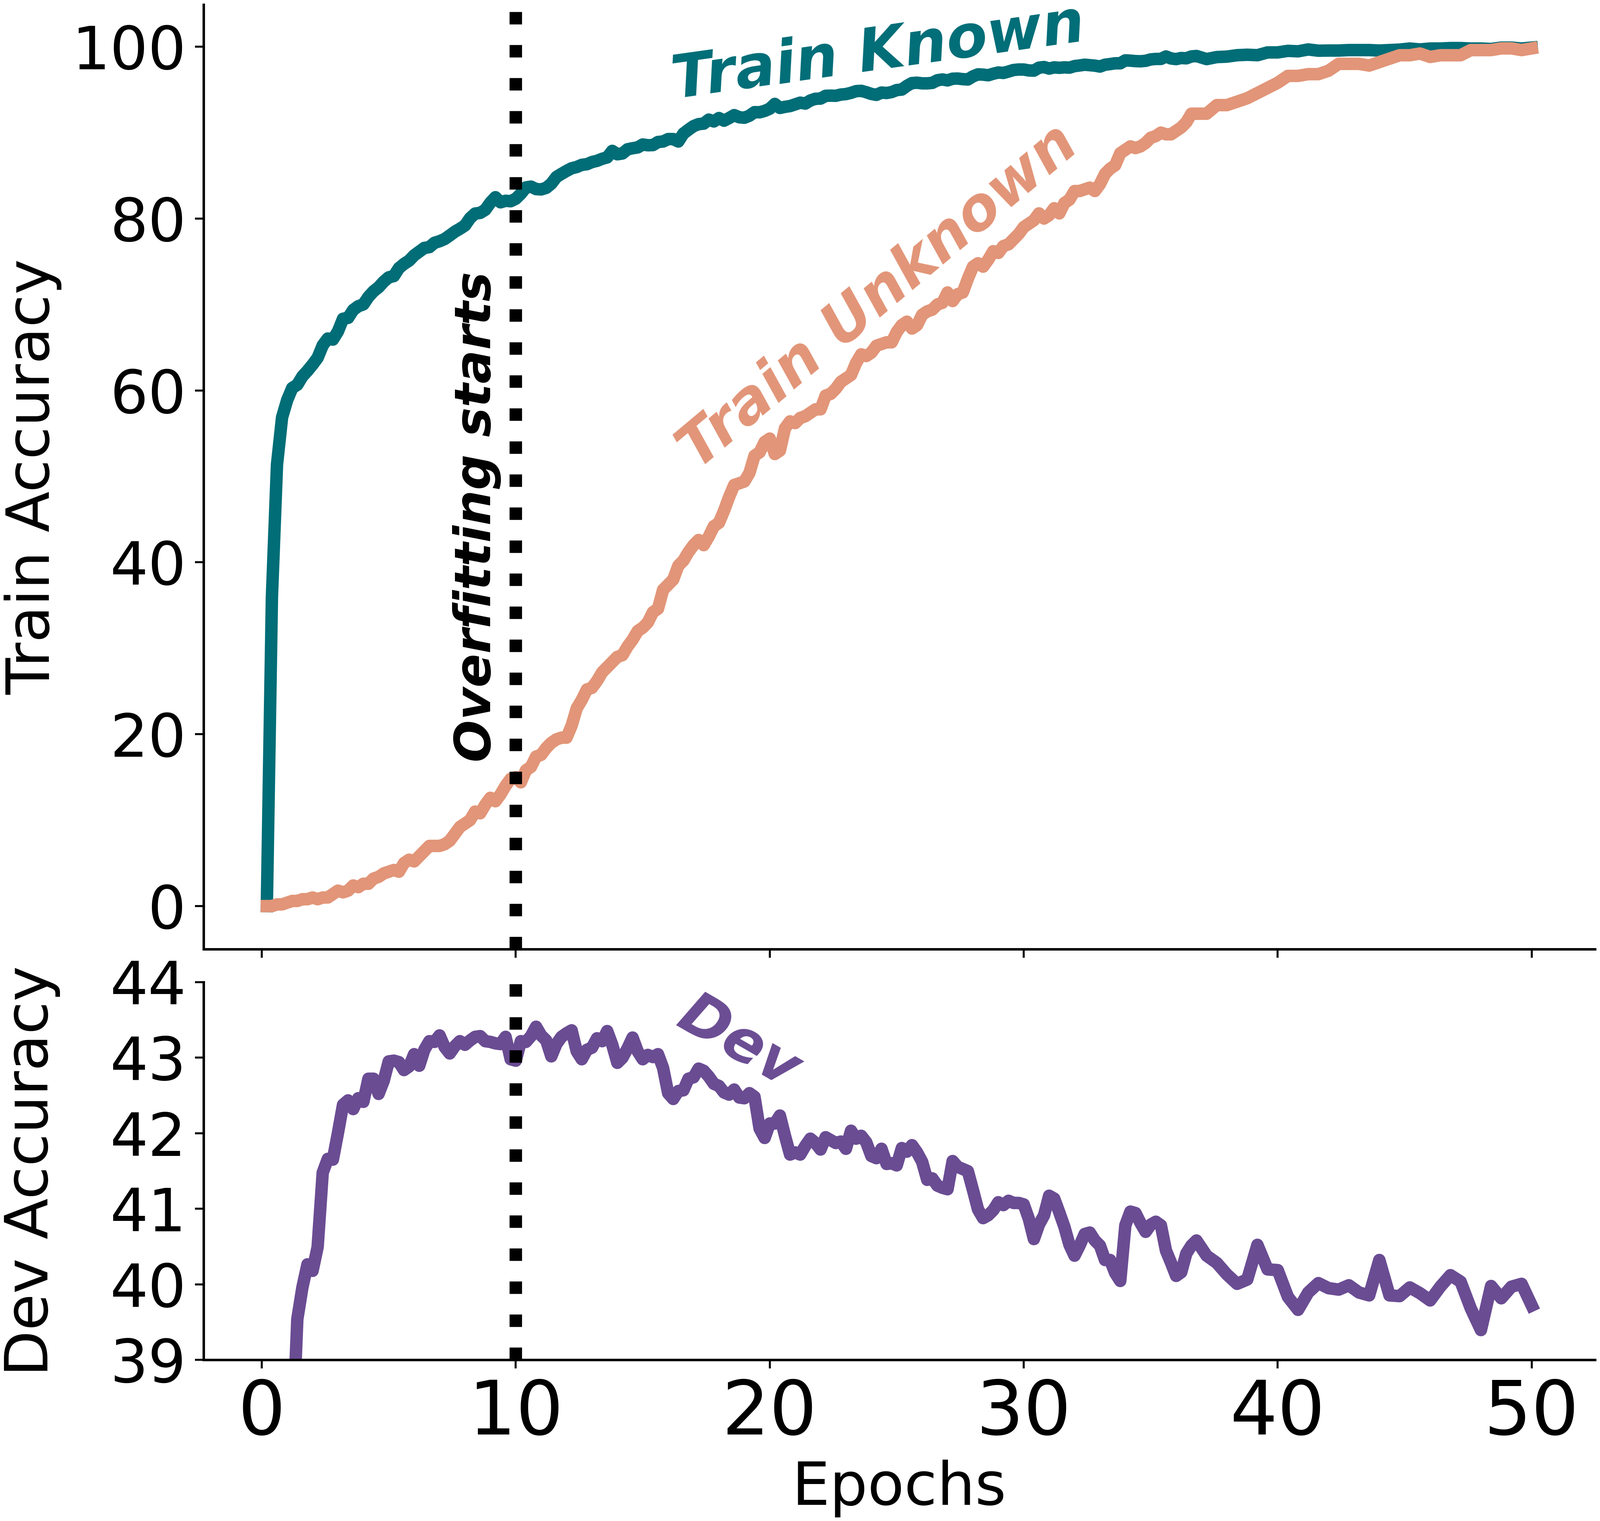
\includegraphics[width=\linewidth,height=0.56\textheight,keepaspectratio]{images/nlp-security-enterprise/gekhman_fig1_unknown_fitted_slower.png}\\[0.2em]
      {\scriptsize Fine-tuning on 50\% Known and 50\% Unknown examples. Gekhman et al., ``Does Fine-Tuning LLMs on New Knowledge Encourage Hallucinations?,'' EMNLP 2024, \href{https://arxiv.org/abs/2405.05904v3}{arXiv:2405.05904v3}, Figure~1.\par}
  \end{columns}
\end{frame}

\begin{frame}{Detecting Hallucination Without a Reference}
  \begin{columns}[T,onlytextwidth]
    \column{0.49\textwidth}
      \begin{itemize}\scriptsize\itemsep0.2em
        \item[\textcolor{red}{$\blacktriangleright$}] \textbf{SelfCheckGPT:} facts the model knows recur across samples; invented details vary. Draw $N$ extra samples $S_1,\dots,S_N$ and score each sentence $r_i$ of the answer with a natural language inference (NLI) model:
          \[ S_{\mathrm{NLI}}(i) = \frac{1}{N}\sum_{n=1}^{N} P(\text{contradict} \mid r_i, S_n). \]
        \item[\textcolor{red}{$\blacktriangleright$}] On 1{,}908 GPT-3 biography sentences with $N = 20$, the area under the precision-recall curve for non-factual sentences is \textbf{92.50} (NLI) and 93.42 (an LLM-prompt variant), against 83.21 for GPT-3's own token probabilities and 72.96 for random.
      \end{itemize}
    \column{0.49\textwidth}
      \begin{itemize}\scriptsize\itemsep0.2em
        \item[\textcolor{red}{$\blacktriangleright$}] \textbf{Semantic entropy:} cluster $M$ sampled answers by bidirectional entailment (A entails B and B entails A), then take the entropy over meanings:
          \[ \mathrm{SE}(x) = -\sum_{c} P(c \mid x)\,\log P(c \mid x), \]
          $x$: the prompt; $c$: a meaning cluster; $P(c \mid x)$: the summed probability of its answers, or their share of the $M$ samples.
        \item[\textcolor{red}{$\blacktriangleright$}] High SE flags \textbf{confabulations}, ``arbitrary and incorrect generations''. Mean AUROC over 30 task--model pairs: \textbf{0.790}, against 0.691 for entropy over strings. Consistent errors go undetected.
      \end{itemize}
  \end{columns}
  \begin{itemize}\scriptsize\itemsep0.2em
    \item[\textcolor{red}{$\blacktriangleright$}] \textbf{Worked example} (answers from Farquhar et al., Fig.~1a): ``Where is the Eiffel Tower?'' sampled six times gives Paris; It's Paris; France's capital Paris; Rome; It's Rome; Berlin. Cluster shares $\tfrac12, \tfrac13, \tfrac16$ give $\mathrm{SE} \approx 1.01$ nats; six rewordings of Paris give $\mathrm{SE} = 0$. Entropy over strings is $\ln 6 \approx 1.79$ in both cases.
    \item[\textcolor{red}{$\blacktriangleright$}] \textbf{Cost:} 10--20 extra generations per answer. Self-consistency keeps the majority answer of such samples; semantic entropy measures how split the vote is.
  \end{itemize}
  {\scriptsize Manakul et al., ``SelfCheckGPT,'' EMNLP 2023, \href{https://arxiv.org/abs/2303.08896v3}{arXiv:2303.08896v3}; Kuhn et al., ``Semantic Uncertainty,'' ICLR 2023, \href{https://arxiv.org/abs/2302.09664v3}{arXiv:2302.09664v3}; Farquhar et al., \textit{Nature} 630, 2024, \href{https://doi.org/10.1038/s41586-024-07421-0}{doi:10.1038/s41586-024-07421-0}.\par}
\end{frame}

\begin{frame}{Chain-of-Verification and Attributed Answers}
  \centering
  \resizebox{\textwidth}{!}{%
  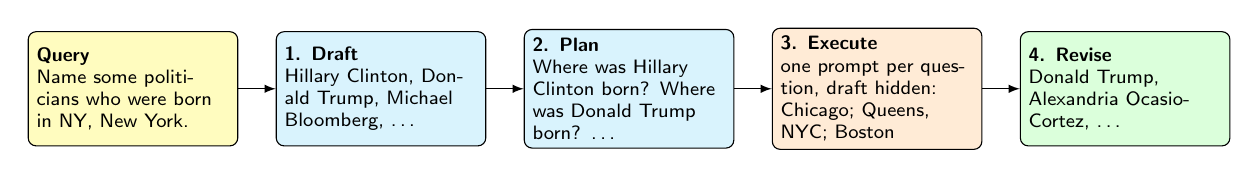
\begin{tikzpicture}[font=\sffamily\scriptsize, >=latex,
      stp/.style={draw, rounded corners=0.1cm, align=left, text width=2.45cm, minimum height=1.45cm, inner sep=3pt},
      qry/.style={stp, fill=yellow!25},
      drf/.style={stp, fill=cyan!15},
      chk/.style={stp, fill=orange!16},
      fin/.style={stp, fill=green!14}]
    \node[qry] (q) at (0,0)     {\textbf{Query}\\Name some politicians who were born in NY, New York.};
    \node[drf] (d) at (3.15,0)  {\textbf{1. Draft}\\Hillary Clinton, Donald Trump, Michael Bloomberg, \ldots};
    \node[drf] (p) at (6.3,0)   {\textbf{2. Plan}\\Where was Hillary Clinton born? Where was Donald Trump born? \ldots};
    \node[chk] (e) at (9.45,0)  {\textbf{3. Execute}\\one prompt per question, draft hidden: Chicago; Queens, NYC; Boston};
    \node[fin] (f) at (12.6,0)  {\textbf{4. Revise}\\Donald Trump, Alexandria Ocasio-Cortez, \ldots};
    \draw[->] (q) -- (d);
    \draw[->] (d) -- (p);
    \draw[->] (p) -- (e);
    \draw[->] (e) -- (f);
  \end{tikzpicture}}\\[0.2em]
  {\scriptsize Answered apart from the draft, the questions expose two wrong names. Example after Dhuliawala et al., Figure~1.\par}
  \vspace{0.2em}
  \begin{columns}[T,onlytextwidth]
    \column{0.49\textwidth}
      \begin{itemize}\scriptsize\itemsep0.3em
        \item[\textcolor{red}{$\blacktriangleright$}] \textbf{Chain-of-Verification (CoVe):} one LLM drafts, plans verification questions, answers them, and revises. In the factored variant each question goes to its own prompt without the draft, so the model cannot copy its own error; factor+revise adds one cross-check prompt per question that compares its answer with the draft.
        \item[\textcolor{red}{$\blacktriangleright$}] Llama 65B biographies: FActScore rises from 55.9 to \textbf{71.4} with factor+revise. On Wikidata list questions, precision rises from 0.17 to 0.36 (two-step variant; factored: 0.32). No retrieval is involved: the model checks itself.
      \end{itemize}
    \column{0.49\textwidth}
      \begin{itemize}\scriptsize\itemsep0.3em
        \item[\textcolor{red}{$\blacktriangleright$}] \textbf{Attributed generation:} answer from retrieved passages and cite one or more of them for each statement. ALCE (Automatic LLMs' Citation Evaluation) scores citation recall (citation support: do the cited passages entail the statement?) and citation precision (is any citation irrelevant?) with NLI.
        \item[\textcolor{red}{$\blacktriangleright$}] ChatGPT on ASQA reaches citation recall \textbf{73.6} with passages in its prompt, but 26.7 when it answers closed-book and a passage is attached afterwards. On ELI5 the best models ``lack complete citation support 50\% of the time.''
      \end{itemize}
  \end{columns}
  \vspace{0.1em}
  {\scriptsize Dhuliawala et al., ``Chain-of-Verification Reduces Hallucination in Large Language Models,'' Findings of ACL 2024, \href{https://aclanthology.org/2024.findings-acl.212/}{aclanthology.org/2024.findings-acl.212}; Gao et al., ``Enabling Large Language Models to Generate Text with Citations,'' EMNLP 2023, \href{https://arxiv.org/abs/2305.14627v2}{arXiv:2305.14627v2}.\par}
\end{frame}

\begin{frame}{Abstention and Where Each Mitigation Acts}
  \begin{columns}[T,onlytextwidth]
    \column{0.50\textwidth}
      \begin{itemize}\scriptsize\itemsep0.25em
        \item[\textcolor{red}{$\blacktriangleright$}] \textbf{Why models guess:} under binary grading (1 point if right, 0 if wrong or ``I don't know''), abstaining never pays. Nine of the 10 popular benchmarks Kalai et al.\ audit grade this way.
        \item[\textcolor{red}{$\blacktriangleright$}] \textbf{Abstention:} decline when $q$, the probability that the answer is right, is below a target $t$. Scored as in the box, answering earns $q - (1-q)\,\frac{t}{1-t}$ in expectation, which is positive exactly when $q > t$.
      \end{itemize}
    \column{0.48\textwidth}
      \begin{tcolorbox}[colframe=KAred, colback=gray!6, boxrule=0.5pt, left=4pt, right=4pt, top=3pt, bottom=3pt]
        \scriptsize Answer only if you are $>t$ confident, since mistakes are penalized $t/(1-t)$ points, while correct answers receive 1 point, and an answer of ``I don't know'' receives 0 points.
      \end{tcolorbox}
      % Kalai et al. also print "t = 0.75 (penalty 2)", but t/(1-t) = 3 at t = 0.75; only values that agree with the formula are quoted.
      {\scriptsize The instruction Kalai et al.\ propose adding to each question; $t = 0.9$ makes a wrong answer cost 9 points. SimpleQA's not-attempted grade records the same behaviour.\par}
  \end{columns}
  \vspace{0.3em}
  {\centering\scriptsize
  \begin{tabular}{>{\raggedright\arraybackslash}p{1.7cm} >{\raggedright\arraybackslash}p{7.4cm} >{\raggedright\arraybackslash}p{3.0cm}}
    \toprule
    \textbf{Stage} & \textbf{Method, and its evidence} & \textbf{Extra inference cost} \\
    \midrule
    SFT data & drop Unknown examples or stop early (Gekhman et al.) & none \\
    Decoding & DoLa (Decoding by Contrasting Layers): final-layer minus early-layer log-probabilities; TruthfulQA $+$12--17 points (LLaMA) & latency $\times$1.01--1.08 \\
    Context & attributed generation from retrieved passages (ALCE) & retrieval, longer prompt \\
    Generation & CoVe factor+revise: FActScore 55.9 $\to$ 71.4 & $2n{+}2$ calls for $n$ questions \\
    Detection & SelfCheckGPT or semantic entropy: flag or withhold & 10--20 samples \\
    Answer policy & abstain below a stated target $t$ & none; fewer answers \\
    \bottomrule
  \end{tabular}\par}
  \vspace{0.1em}
  {\scriptsize Kalai et al., \href{https://arxiv.org/abs/2509.04664v1}{arXiv:2509.04664v1}, Section~4 and Table~2; Chuang et al., ``DoLa: Decoding by Contrasting Layers Improves Factuality in Large Language Models,'' ICLR 2024, \href{https://arxiv.org/abs/2309.03883v2}{arXiv:2309.03883v2}.\par}
\end{frame}
